\section{Relevant Figures}

This section includes any figures relevant to the project. It has the PCA results, and the ROC curves for our model, as well as a comparison of performance for the Random Forest algorithm

\begin{figure}[H] %h forces the figure to be inserted right here
    \centering
    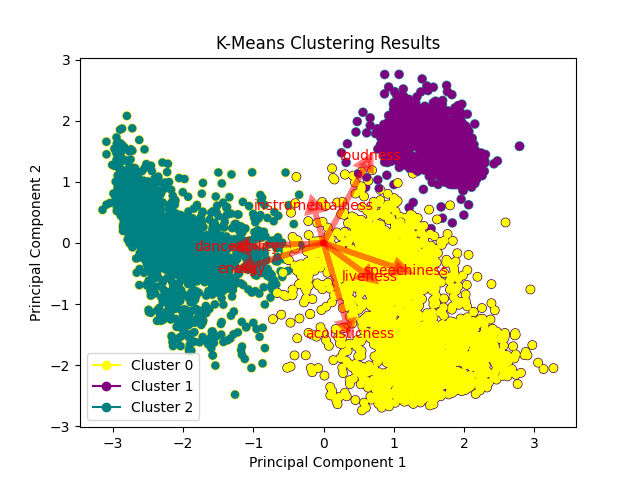
\includegraphics[width=0.75\linewidth]{figs/kmeanscluster.png}
    \caption{Clustering PCA Results}
    \vspace{-8mm}
\end{figure}

%Here are the ROC curves for the algorithms created for this project.

\begin{figure}[H] %h forces the figure to be inserted right here
    \centering
    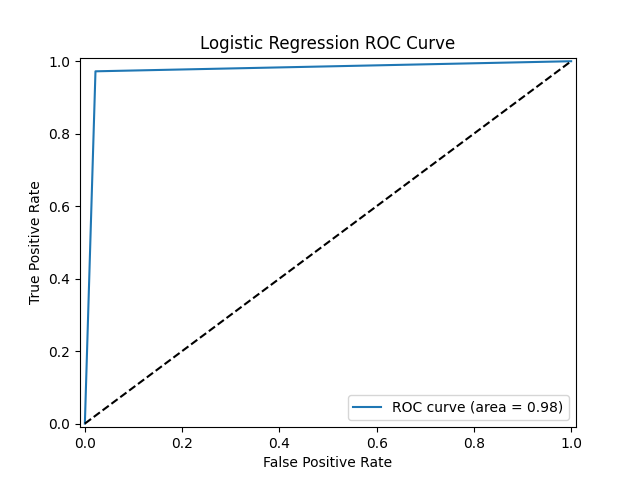
\includegraphics[width=0.75\linewidth]{figs/logistic-regressionROC.png}
    \caption{Logistic Regression ROC}
    \vspace{-8mm}
\end{figure}

\begin{figure}[H] %h forces the figure to be inserted right here
    \centering
    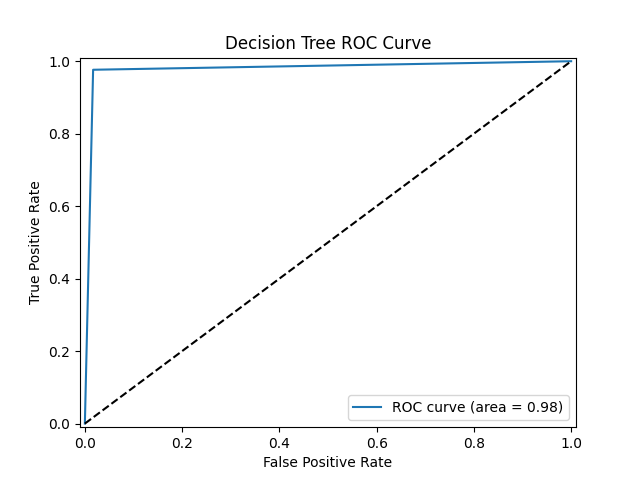
\includegraphics[width=0.75\linewidth]{figs/decision-treeROC.png}
    \caption{Decision Tree ROC}
    \vspace{-8mm}
\end{figure}

% \begin{figure}[H] %h forces the figure to be inserted right here
%     \centering
%     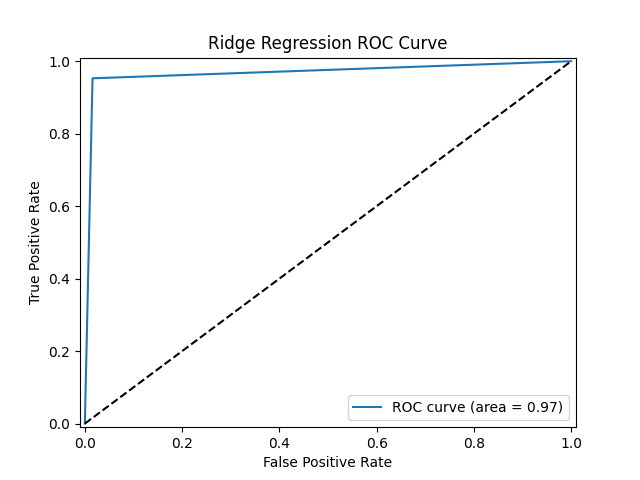
\includegraphics[width=0.75\linewidth]{figs/scikitridgeROC.png}
%     \caption{Ridge Regression ROC}
%     \vspace{-7mm}
% \end{figure}

% \begin{figure}[H] %h forces the figure to be inserted right here
%     \centering
%     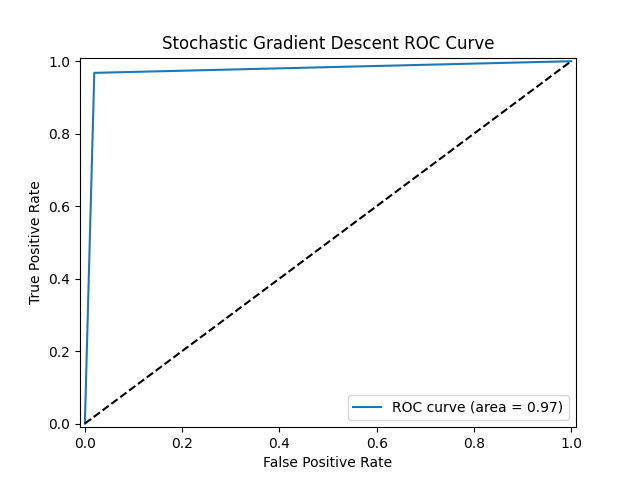
\includegraphics[width=0.75\linewidth]{figs/scikitSGD-ROC.png}
%     \caption{Stochastic Gradient Descent ROC}
%     \vspace{-4mm}
% \end{figure}

\begin{figure}[H] %h forces the figure to be inserted right here
    \centering
    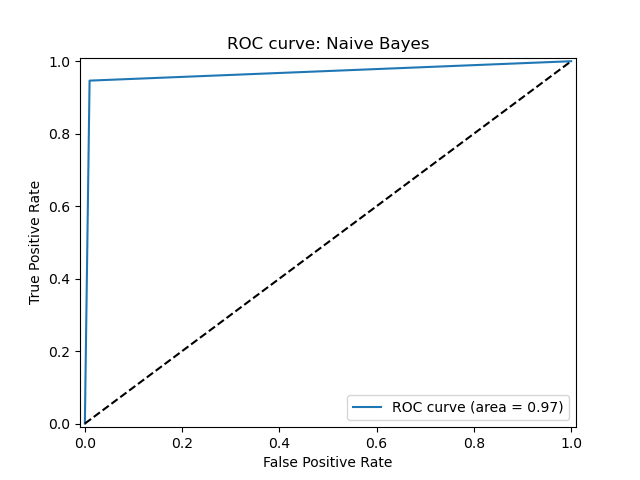
\includegraphics[width=0.75\linewidth]{figs/naive-bayes-ROC.png}
    \caption{Naive Bayes ROC}
    \vspace{-8mm}
\end{figure}

\begin{figure}[H] %h forces the figure to be inserted right here
    \centering
    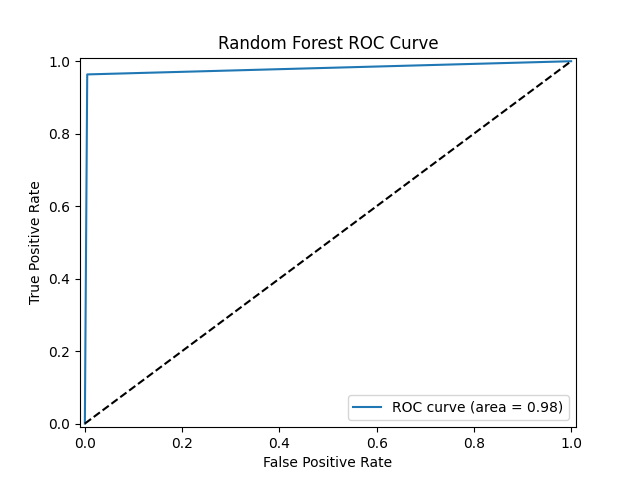
\includegraphics[width=0.75\linewidth]{figs/random-forest-ROC.png}
    \caption{Random Forest ROC}
    \vspace{-8mm}
\end{figure}

% \begin{figure}[H] %h forces the figure to be inserted right here
%     \centering
%     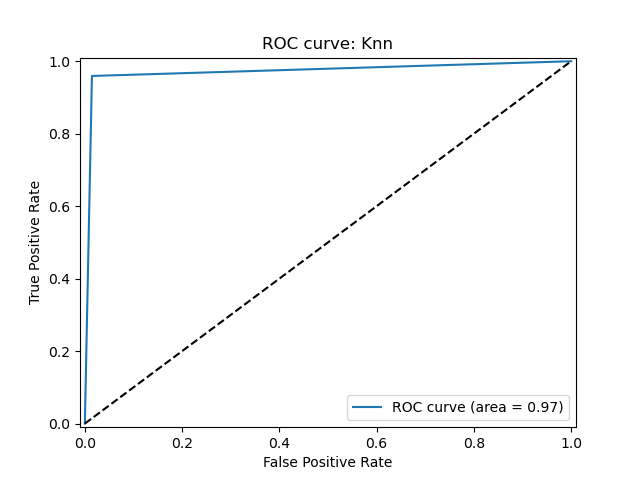
\includegraphics[width=0.75\linewidth]{figs/knn-ROC.png}
%     \caption{K-NN ROC}
%     \vspace{-4mm}
% \end{figure}

% \begin{figure}[H] %h forces the figure to be inserted right here
%     \centering
%     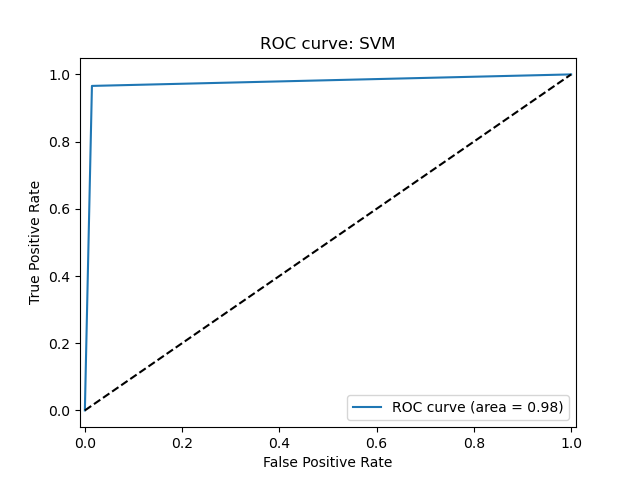
\includegraphics[width=0.75\linewidth]{figs/svm-ROC.png}
%     \caption{SVM ROC}
%     \vspace{-4mm}
% \end{figure}

%Here is the  Random Forest result with depth = 10, and number of trees from 10 to 100

\begin{figure}[H] %h forces the figure to be inserted right here
    \centering
    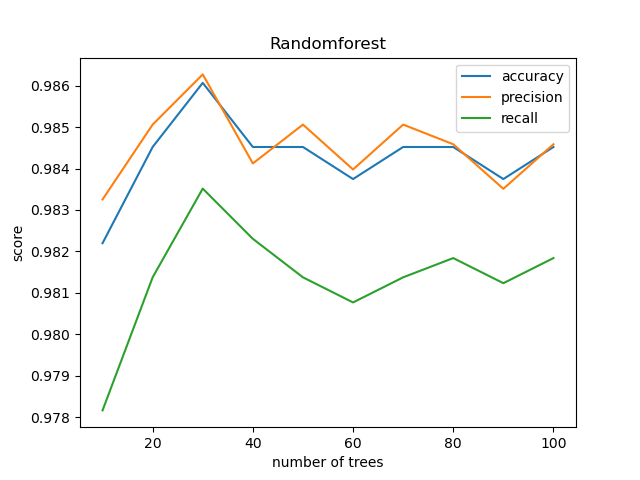
\includegraphics[width=0.75\linewidth]{figs/randomforest_scores(final).png}
    \caption{Result of Random Forest}
    \vspace{-7.5mm}
\end{figure}

% Here is the performance of K-NN with different number of neighbors from 1 to 100 

% \begin{figure}[H] %h forces the figure to be inserted right here
%     \centering
%     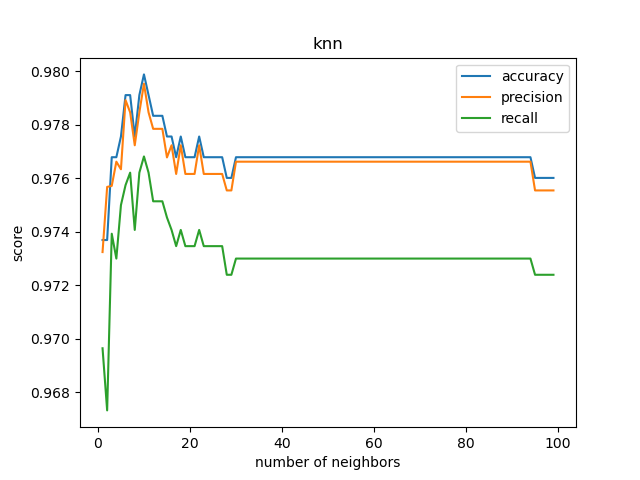
\includegraphics[width=0.75\linewidth]{figs/knn_scores.png}
%     \caption{Result of K-NN}
%     \vspace{-7mm}
% \end{figure}
